% *********************************************************************
% © 2021–2024 Jeremy Sylvestre
%
% Permission is granted to copy, distribute and/or modify this document
% under the terms of the GNU Free Documentation License, Version 1.3 or
% any later version published by the Free Software Foundation; with no
% Invariant Sections, no Front-Cover Texts, and no Back-Cover Texts. A
% copy of the license is included in the appendix entitled “GNU Free
% Documentation License” that appears in the output document of this
% PreTeXt source code. All trademarks™ are the registered® marks of
% their respective owners.
%
% *********************************************************************

\newcommand*{\xmin}{-0.5}
\newcommand*{\xmax}{5}
\newcommand*{\ymin}{-0.5}
\newcommand*{\ymax}{2.5}

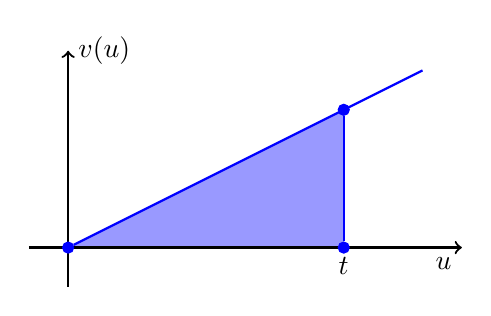
\begin{tikzpicture}
[
	closedpt/.style={circle,draw,fill,inner sep=0pt,minimum size=4pt},
	openpt/.style={circle,draw,inner sep=0pt,minimum size=4pt}
]

	% fills
	\fill[blue!40!white] (0,0) -- (3.5,1.75) -- (3.5,0) -- cycle;

	% axes
	\draw[->,thick] (\xmin,0) -- (\xmax,0) node[below left] {$u$};
	\draw[->,thick] (0,\ymin) -- (0,\ymax) node[right] {$v(u)$};

	% line
	\node[blue,closedpt] at (0,0) (start) {};
	\node[blue,closedpt] at (3.5,1.75) (stop) {};
	\node[blue,closedpt] at (3.5,0) (dend) {};
	\node[below] at (3.5,0) {$t$};
	\draw[blue,thick] (start) -- (4.5,2.25);
	\draw[blue,thick] (stop) -- (dend);

\end{tikzpicture}
